\documentclass[12pt,letterpaper]{article}
\usepackage[utf8]{inputenc}
\usepackage[spanish]{babel}
\usepackage{graphicx}
\usepackage[left=2cm,right=2cm,top=2cm,bottom=2cm]{geometry}
\usepackage{graphicx} % figuras
% \usepackage{subfigure} % subfiguras
\usepackage{float} % para usar [H]
\usepackage{amsmath}
%\usepackage{txfonts}
\usepackage{stackrel} 
\usepackage{multirow}
\usepackage{enumerate} % enumerados
\renewcommand{\labelitemi}{$-$}
\renewcommand{\labelitemii}{$\cdot$}
% \author{}
% \title{Caratula}
\begin{document}

% Fancy Header and Footer
% \usepackage{fancyhdr}
% \pagestyle{fancy}
% \cfoot{}
% \rfoot{\thepage}
%

% \usepackage[hidelinks]{hyperref} % CREA HYPERVINCULOS EN INDICE

% \author{}
\title{Caratula}

\begin{titlepage}
\begin{center}
\large{UNIVERSIDAD PRIVADA DE TACNA}\\
\vspace*{-0.025in}
\begin{figure}[htb]
\begin{center}

\includegraphics[width=8cm]{./Imagenes/logo}
\end{center}
\end{figure}
\vspace*{0.15in}
INGENIERIA DE SISTEMAS  \\

\vspace*{0.5in}
\begin{large}
TITULO:\\
\end{large}

\vspace*{0.1in}
\begin{Large}
\textbf{INFORME DE LABORATORIO N2 - PowerBI} \\
\end{Large}

\vspace*{0.3in}
\begin{Large}
\textbf{CURSO:} \\
\end{Large}

\vspace*{0.1in}
\begin{large}
INTELIGENCIA DE NEGOCIOS\\
\end{large}

\vspace*{0.3in}
\begin{Large}
\textbf{DOCENTE(ING):} \\
\end{Large}

\vspace*{0.1in}
\begin{large}
 Patrick Cuadros Quiroga\\
\end{large}

\vspace*{0.2in}
\vspace*{0.1in}
\begin{large}
Alumna: \\
\begin{flushleft}
Salamanca Contreras, Fiorella Rosmery 		\hfill	(2015053237) \\
\end{flushleft}
\end{large}
\end{center}

\end{titlepage}


\tableofcontents % INDICE
\thispagestyle{empty} % INDICE SIN NUMERO
\newpage
\setcounter{page}{1} % REINICIAR CONTADOR DE PAGINAS DESPUES DEL INDICE

\section{Ejercicio 1: Crear relaciones - Tarea 1: Relaciones Automáticas} 


\begin{enumerate}[1.]
    \item Ingresar a Power BI Desktop.
    \item En la Ventana de Power BI Desktop, click en Obtener Datos (Get Data)

	\begin{center}
	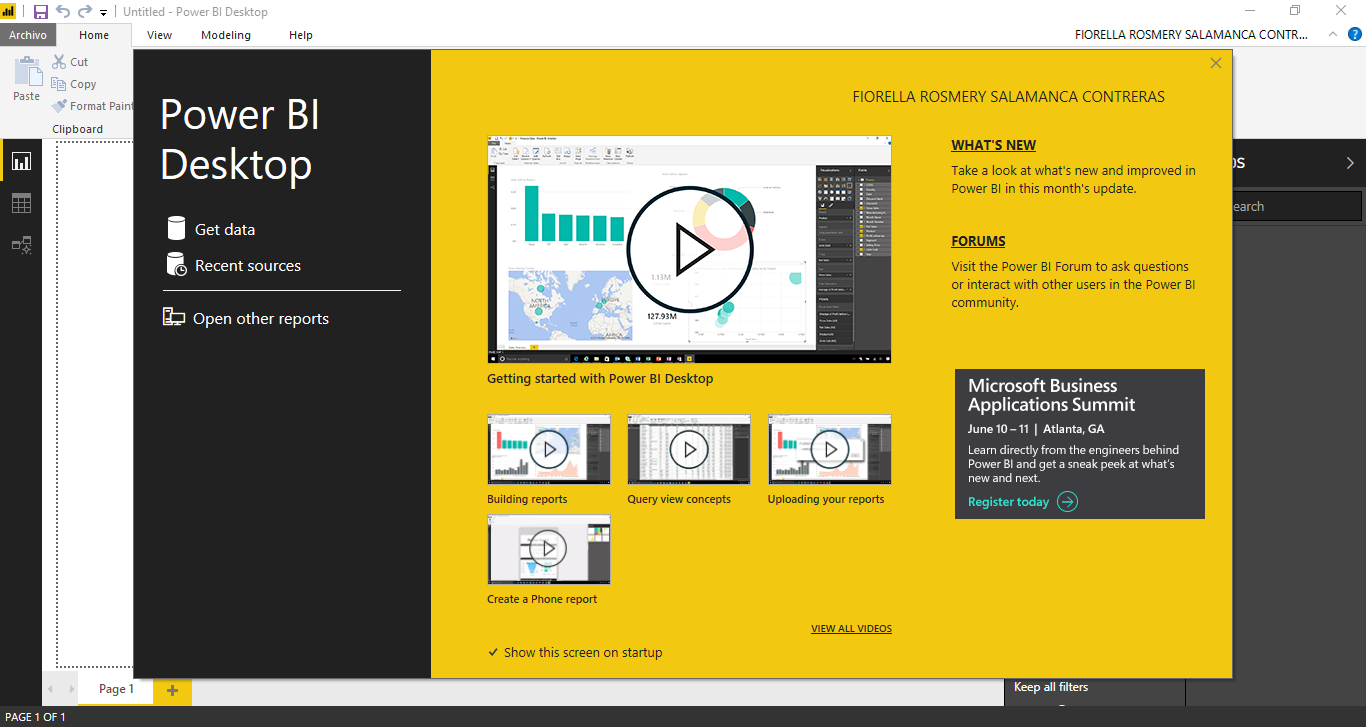
\includegraphics[width=17cm]{./Imagenes/Ejercicio1-Tarea1/1}
	\end{center}	

    \item En el cuadro de dialogo Obtener Datos (Get Data), asegurarse que Excel esta seleccionado y hacer click
en Conectar (Connect).

	\begin{center}
	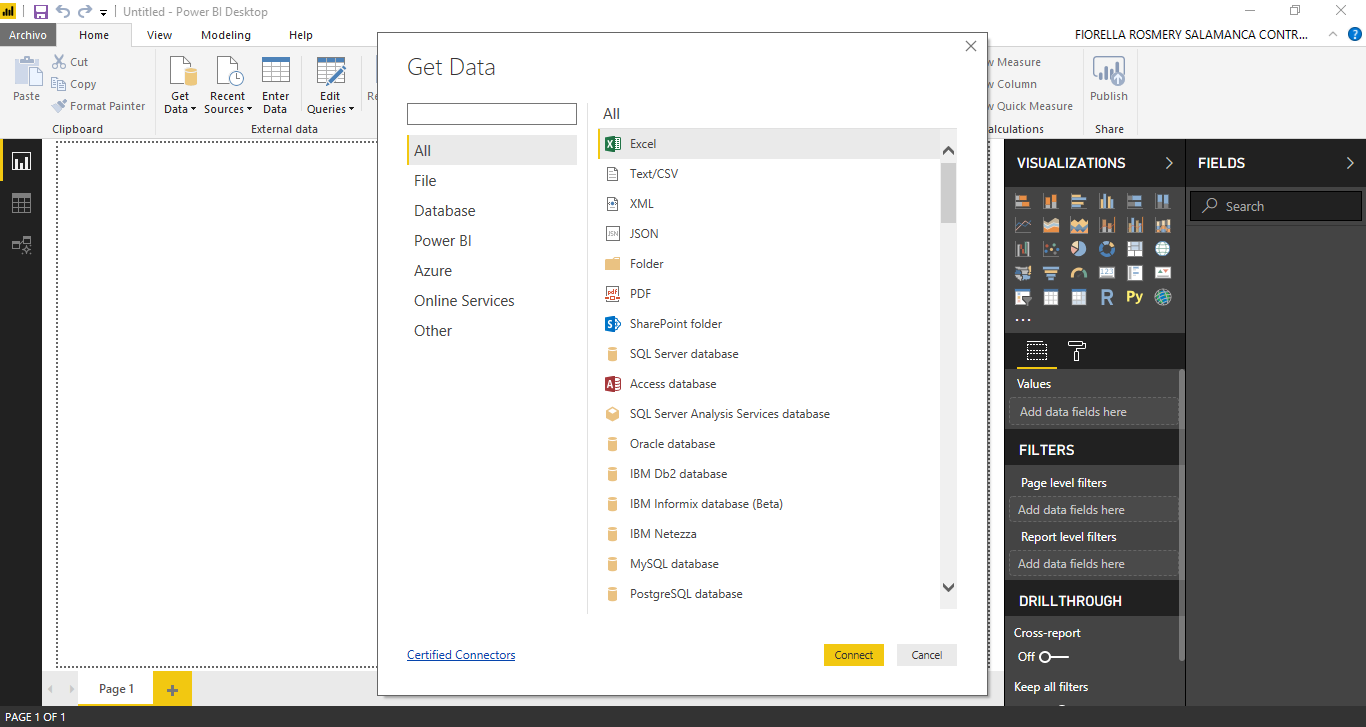
\includegraphics[width=17cm]{./Imagenes/Ejercicio1-Tarea1/2}
	\end{center}	

    \item  En el cuadro de dialogo Abrir (Open), buscar el archivo Adventure Works Sales Data.xlsx, y luego hacer
click en Abrir (Open).

	\begin{center}
	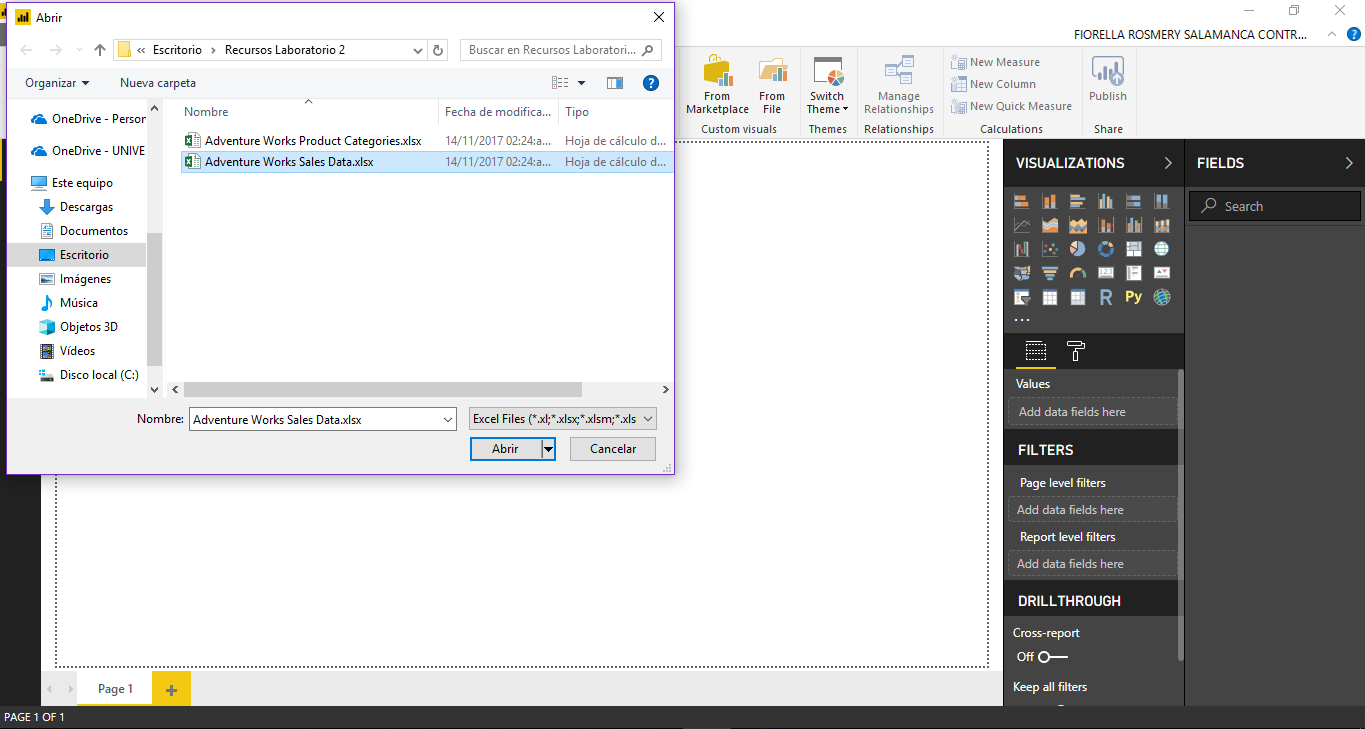
\includegraphics[width=17cm]{./Imagenes/Ejercicio1-Tarea1/33}
	\end{center}	

    \item En el cuadro de dialogo Explorador (Navigator), seleccionar las hojas DimCurrency, DimCustomer,
DimDate, DimProduct, DimPromotion, DimSalesTerritory, y FactInternetSales.
    \item Hacer click en Cargar (Load).

	\begin{center}
	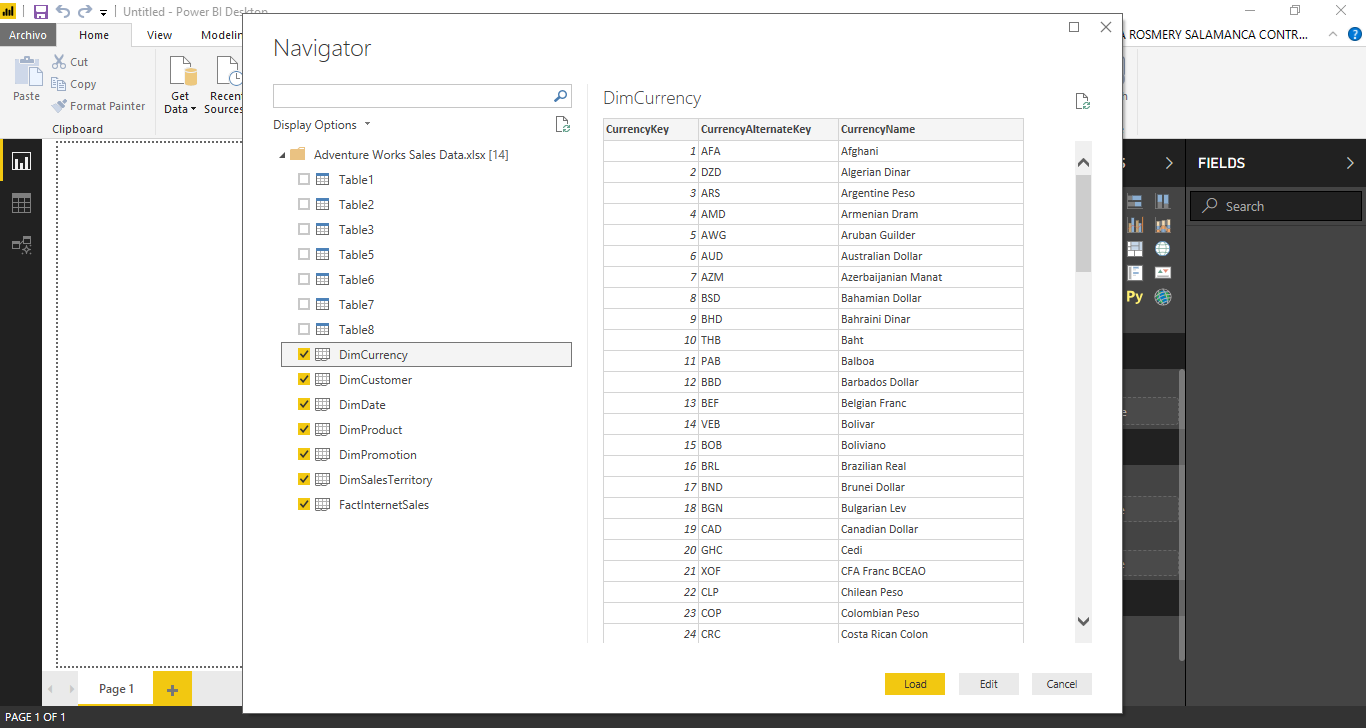
\includegraphics[width=17cm]{./Imagenes/Ejercicio1-Tarea1/3}
	\end{center}	

    \item En el panel de vistas a mano derecho, hacer click en Relaciones (Relationships).
    \item En el menú principal, hacer click en Administrar relaciones (Manage Relationships).
    \item En el cuadro de Administrar relaciones (Manage Relationships), hacer click en Nueva (New).
    \item  En el cuadro de Administrar relaciones (Manage Relationships), en la lista de tablas superior, hacer click
en FactInternetSales. Cuando la vista previa de la table aparezca hacer click en la columna
OrderDateKey.
    \item En la lista de table inferior, hacer click en DimDate. Cuando la vista previa de la table aparezca hacer click
en la columna DateKey.
    \item Revisar que la cardinalidad (Cardinality) esta seleccionada para Muchos a Uno (Many to One (*:1)), que la
Dirección del filtro cruzado (Cross filter direction) es Sencilla (Single), y que la opción Hacer esta relación
activa (Make this relationship active) se encuentra seleccionada, luego hacer click en Aceptar (OK).

	\begin{center}
	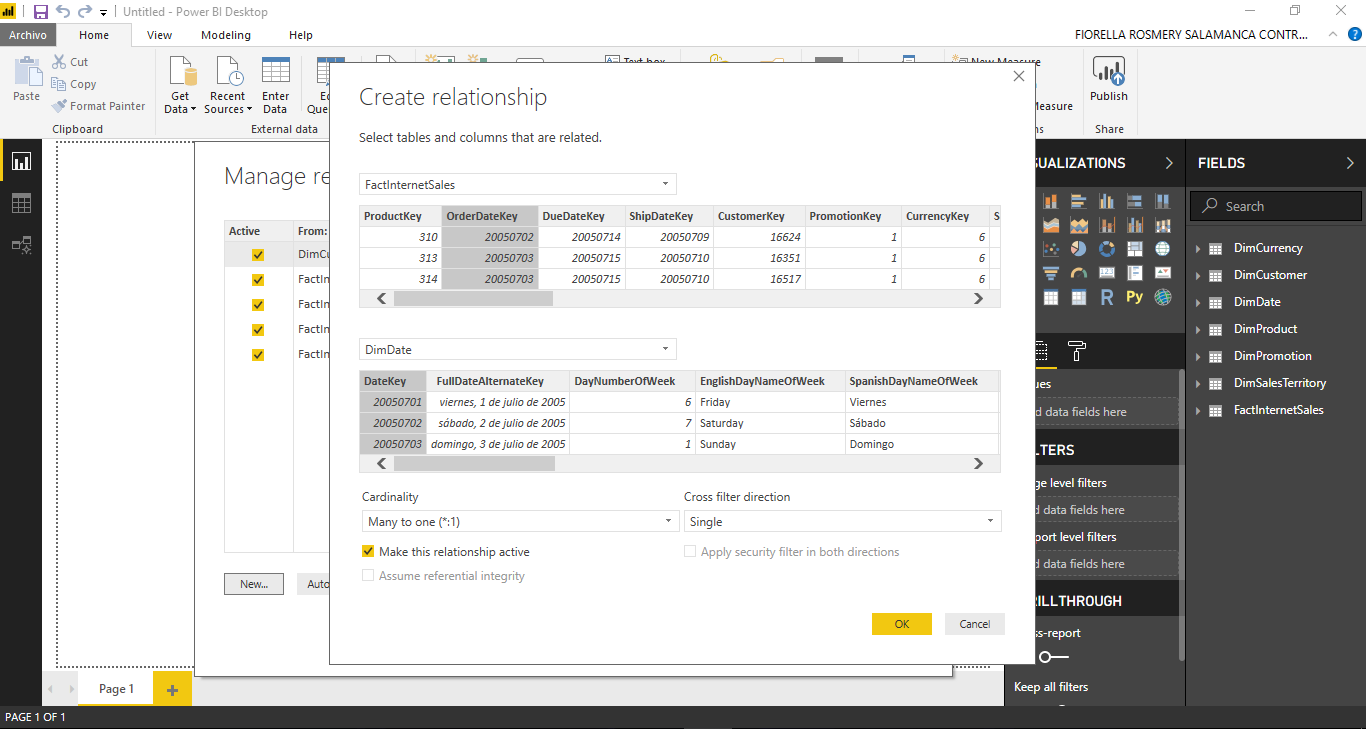
\includegraphics[width=17cm]{./Imagenes/Ejercicio1-Tarea1/4}
	\end{center}	

    \item En el cuadro de Administrar relaciones (Manage Relationships), hacer click en Cerrar (Close).
   \item En el diagrama, en la tabla FactInternetSales, hacer click en la columna DueDateKey. Arrastrar la columna
DueDateKey a la columna DateKey de la tabla DimDate.
   \item En el diagrama, en la tabla FactInternetSales, hacer click en la columna ShipDateKey. Arrastrar la
columna ShipDateKey a la columna DateKey de la tabla DimDate.

	\begin{center}
	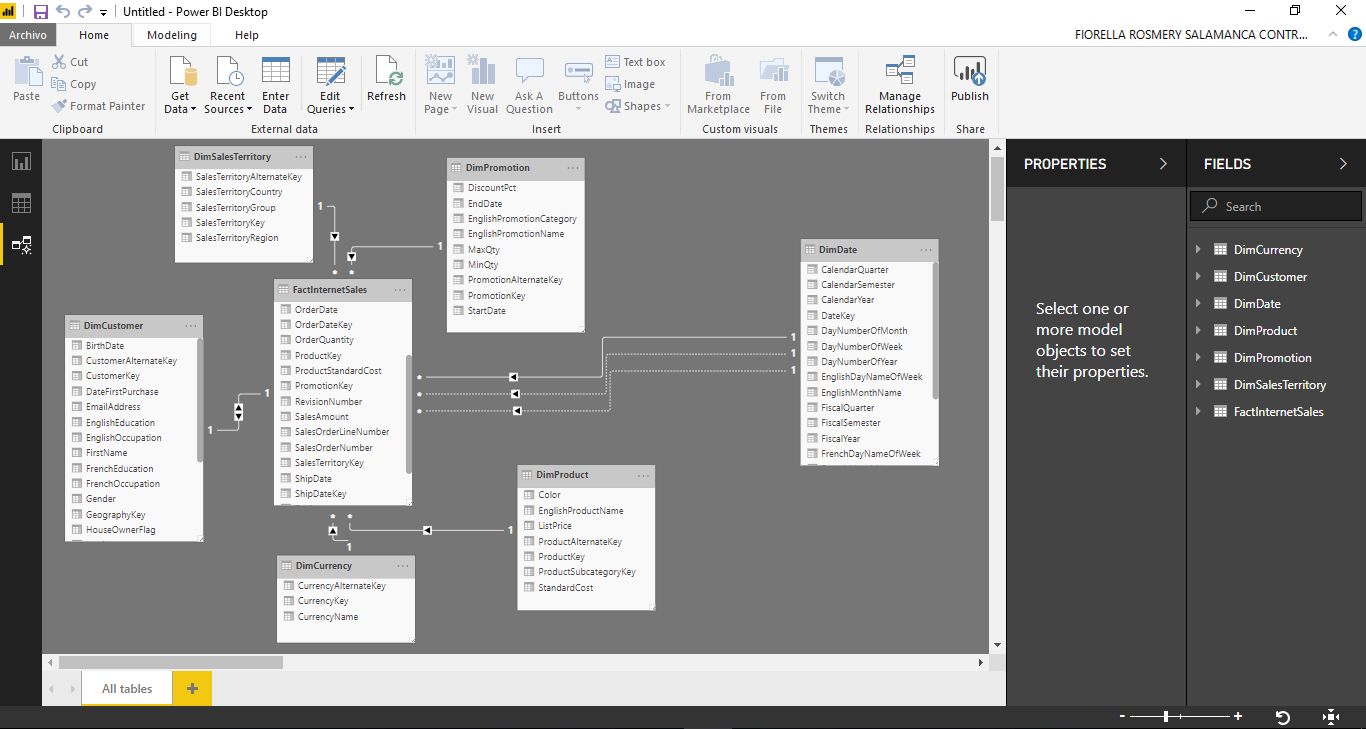
\includegraphics[width=17cm]{./Imagenes/Ejercicio1-Tarea1/5}
	\end{center}	

   \item En el menú principal, hacer click en Administrar relaciones (Manage Relationships).
   \item En el cuadro de Administrar relaciones (Manage Relationships), hacer doble click en la relación
FactInternetSales (CurrencyKey).
   \item En la lista de Dirección de Filtro Cruzado (Cross filter direction), hacer click en Sencilla (Single), luego
hacer click en Aceptar (OK).


	\begin{center}
	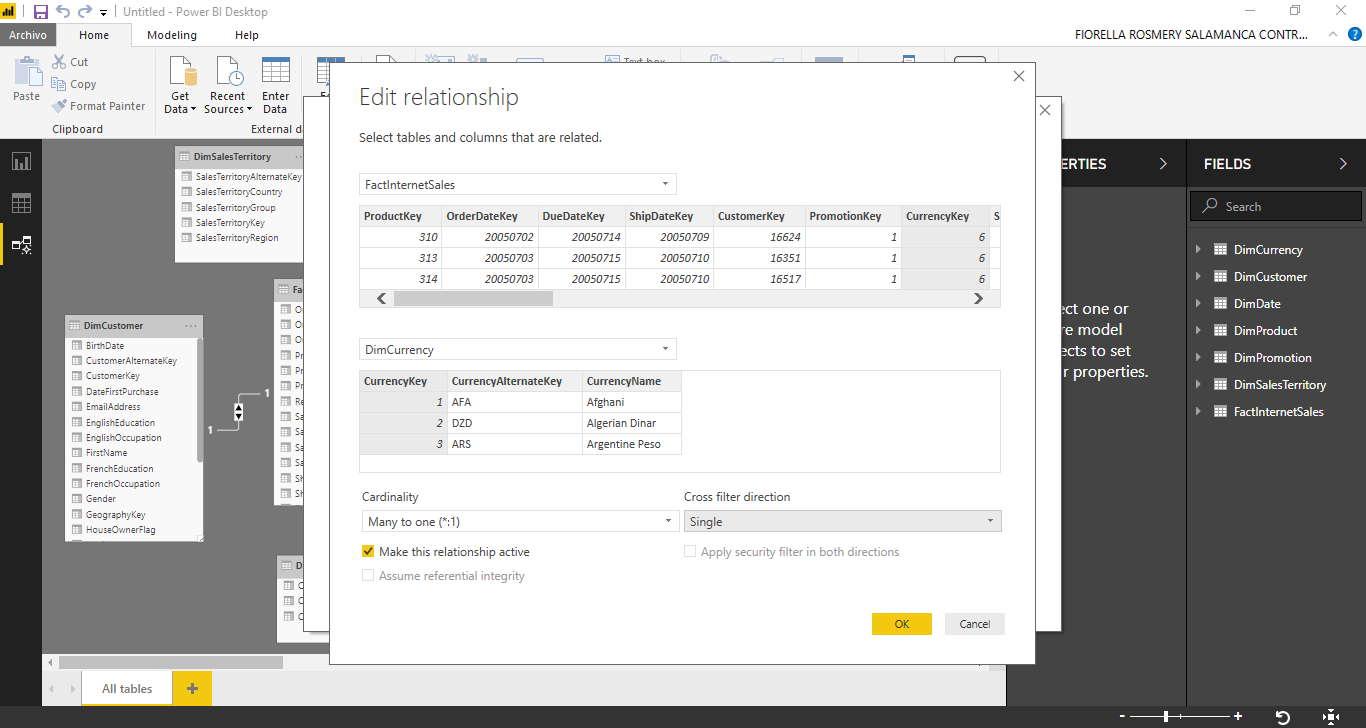
\includegraphics[width=17cm]{./Imagenes/Ejercicio1-Tarea1/6}
	\end{center}	


   \item En el cuadro de Administrar relaciones (Manage Relationships), hacer doble click en la relación
FactInternetSales (ProductKey).
   \item En la lista de Dirección de Filtro Cruzado (Cross filter direction), hacer click en Sencilla (Single), luego
hacer click en Aceptar (OK).


	\begin{center}
	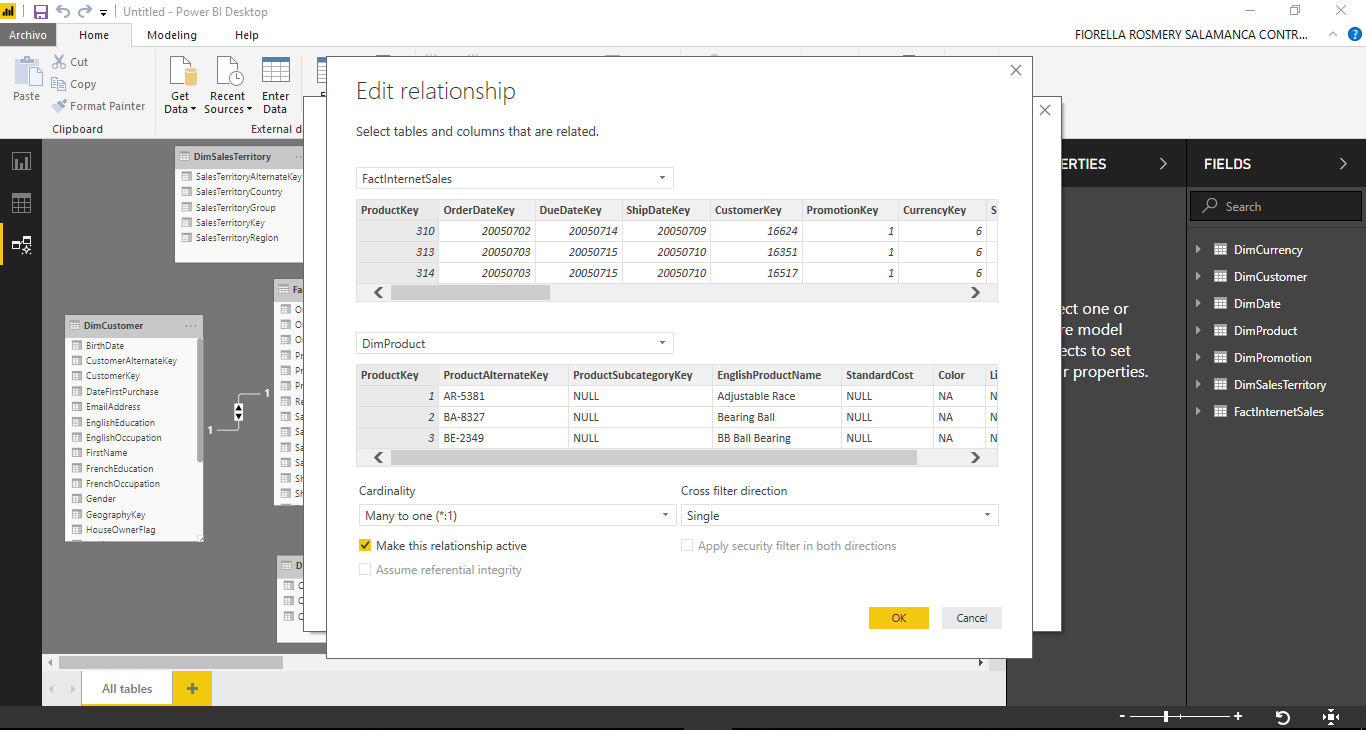
\includegraphics[width=17cm]{./Imagenes/Ejercicio1-Tarea1/7}
	\end{center}	


   \item En el cuadro de Administrar relaciones (Manage Relationships), hacer doble click en la relación
FactInternetSales (PromotionKey).
   \item En la lista de Dirección de Filtro Cruzado (Cross filter direction), hacer click en Sencilla (Single), luego
hacer click en Aceptar (OK).

	\begin{center}
	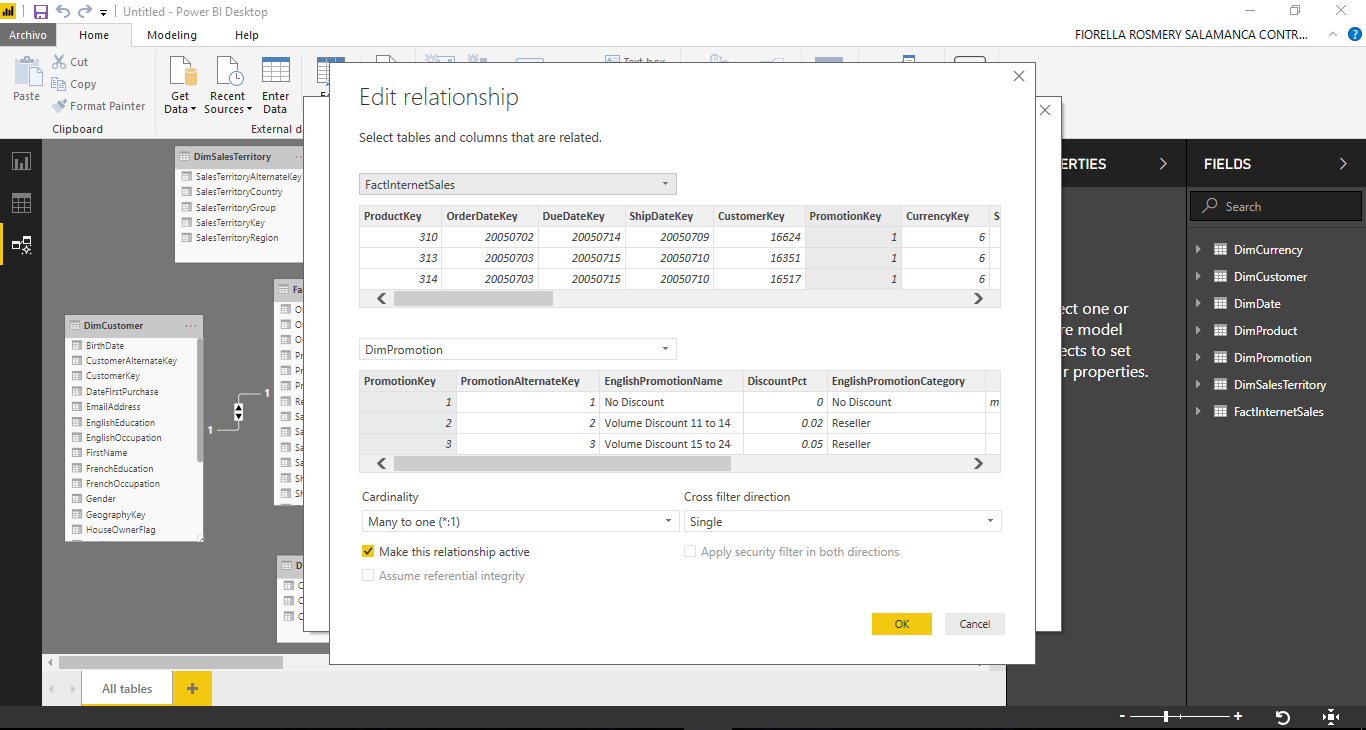
\includegraphics[width=17cm]{./Imagenes/Ejercicio1-Tarea1/8}
	\end{center}	

   \item En el cuadro de Administrar relaciones (Manage Relationships), hacer doble click en la relación
FactInternetSales (SalesTerritoryKey).
   \item En la lista de Dirección de Filtro Cruzado (Cross filter direction), hacer click en Sencilla (Single), luego
hacer click en Aceptar (OK).

	\begin{center}
	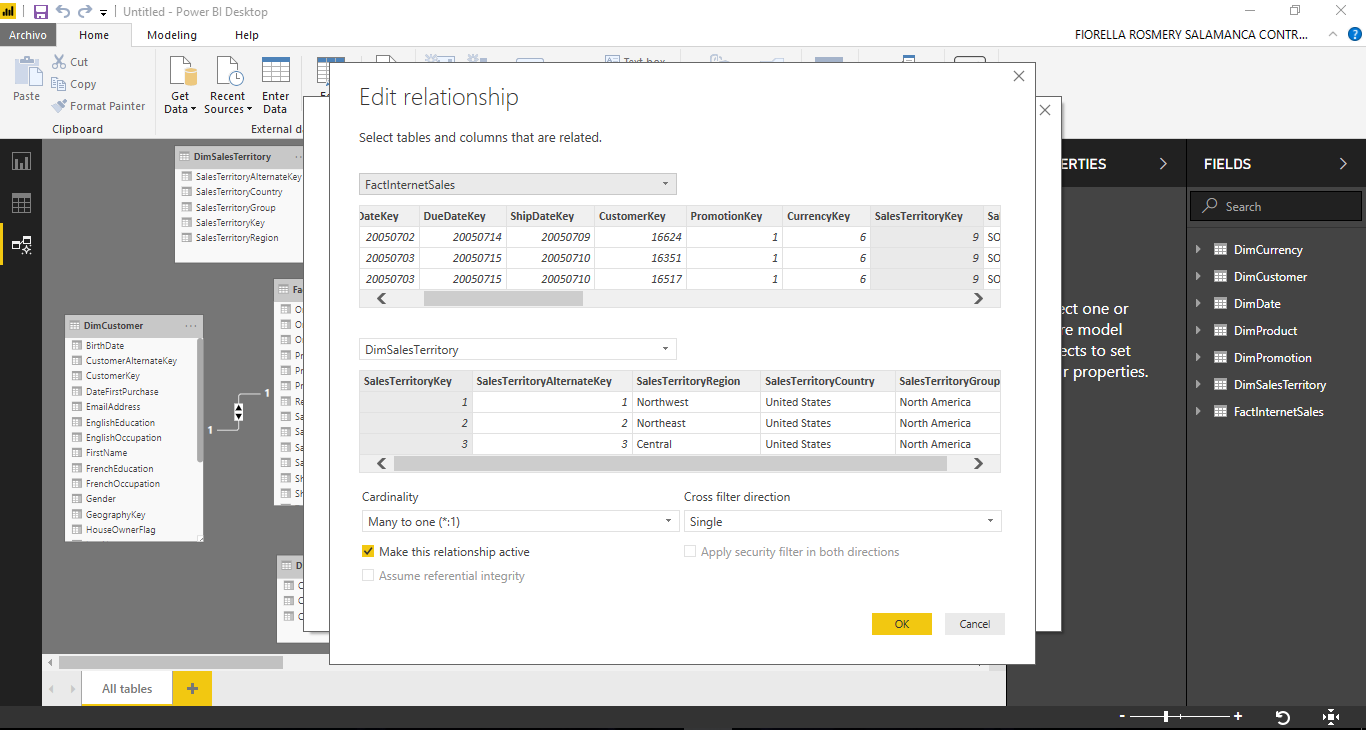
\includegraphics[width=17cm]{./Imagenes/Ejercicio1-Tarea1/9}
	\end{center}	

   \item En el cuadro de Administrar relaciones (Manage Relationships), hacer click en Cerrar (Close)..
   \item Hacer click en la línea de relación entre FactInternetSales and DimCustomer y presionar Borrar (Delete).
   \item En el cuadro de dialogo Eliminar relación (Delete Relationship), hacer click en Borrar (Delete).

	\begin{center}
	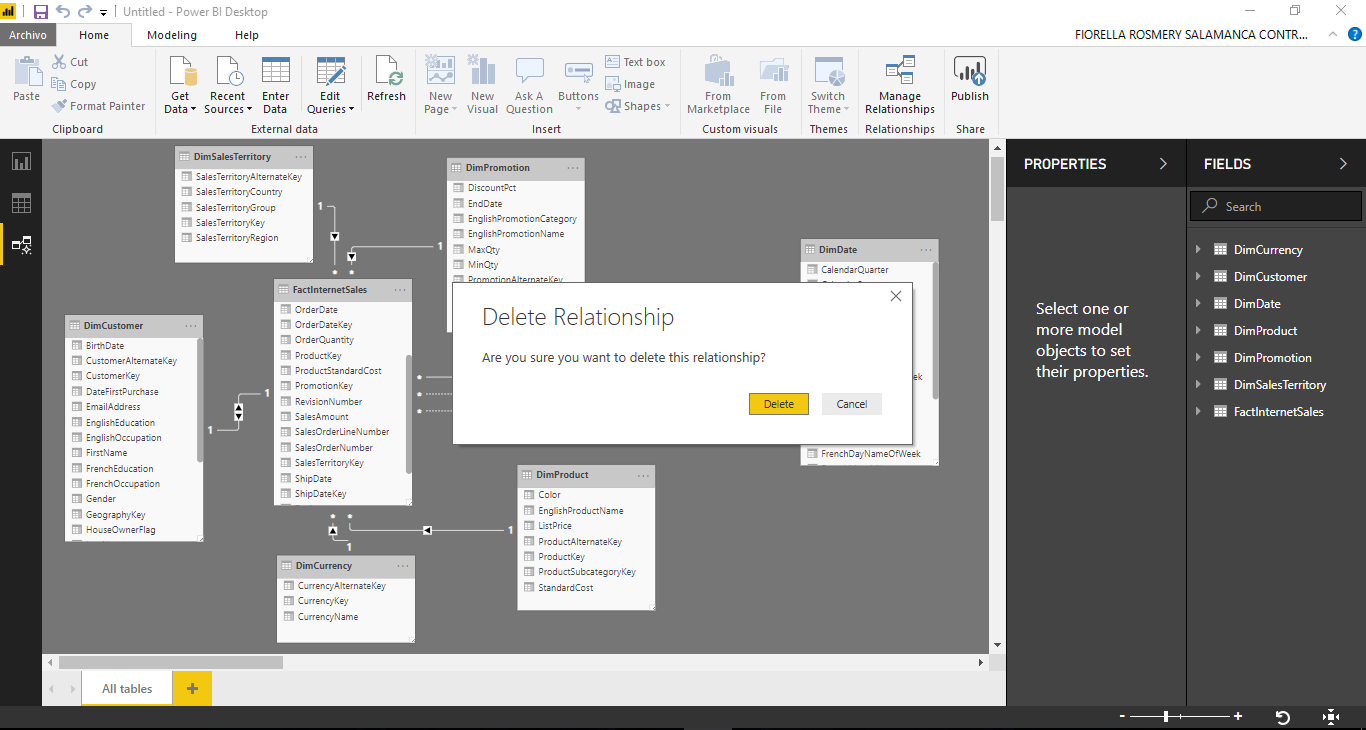
\includegraphics[width=17cm]{./Imagenes/Ejercicio1-Tarea1/10}
	\end{center}	

   \item En el menú principal, hacer click en Administrar relaciones (Manage Relationships).
   \item En el cuadro de Administrar relaciones (Manage Relationships), hacer click en Nueva (New).
   \item En la lista de tablas superior, hacer click en FactInternetSales. Luego hacer click en la columna
CustomerKey en la vista de datos previa.
   \item En la lista de tablas superior, hacer click en DimCustomer, y hacer click CustomerKey en la vista de datos
previa.
   \item En la lista de Cardinalidad (Cardinality), hacer click en Muchos a Uno (Many to One (*:1)), y luego hacer
click en Aceptar (OK).

	\begin{center}
	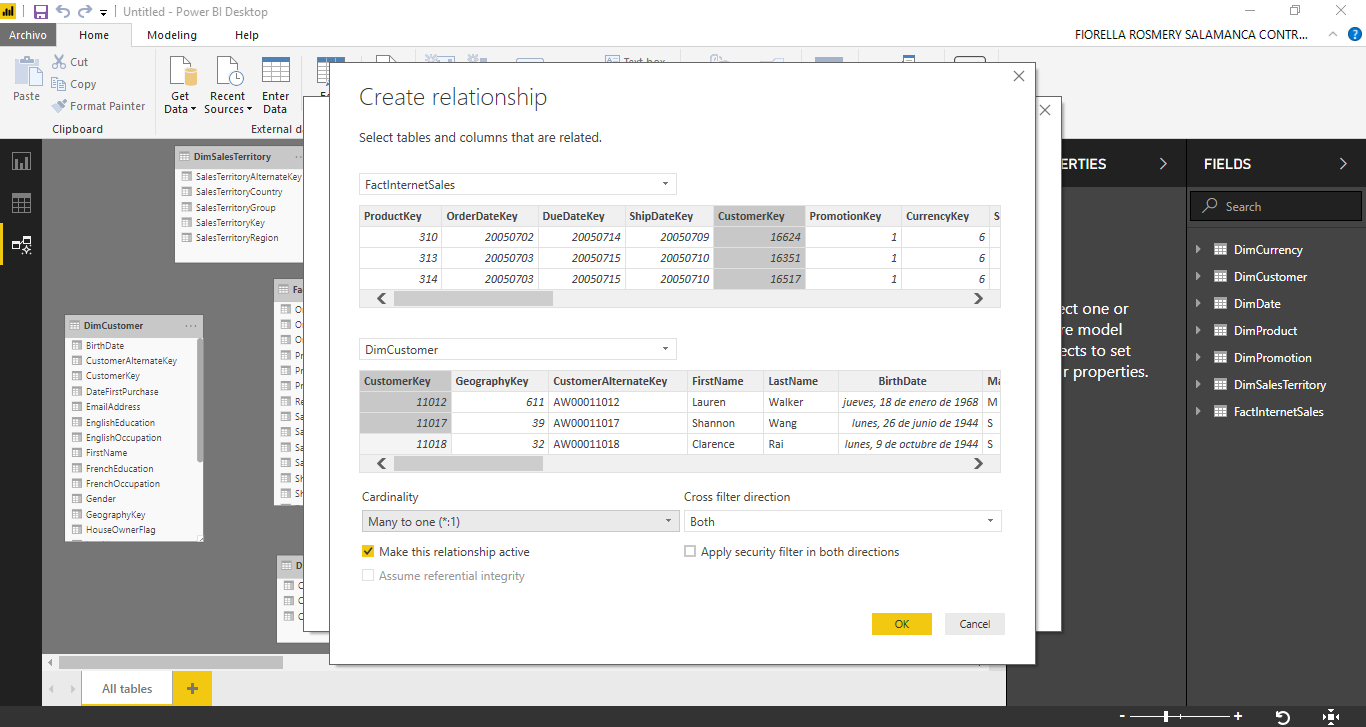
\includegraphics[width=17cm]{./Imagenes/Ejercicio1-Tarea1/11}
	\end{center}	

   \item En el cuadro de Administrar relaciones (Manage Relationships), hacer click en Cerrar (Close).
   \item Hacer click en Guardar (Save), y cuargar el archive como Ventas Adventure Works.pbix.

	\begin{center}
	
\includegraphics[width=5cm]{./Imagenes/Ejercicio1-Tarea1/12}
	\end{center}	

\end{enumerate}



\section{Ejercicio 1: Crear relaciones - Tarea 2: Relaciones Manuales} 


\begin{enumerate}[1.]

    \item En la Ventana de Power BI Desktop, click en Obtener Datos (Get Data) y luego en Excel.

	\begin{center}
	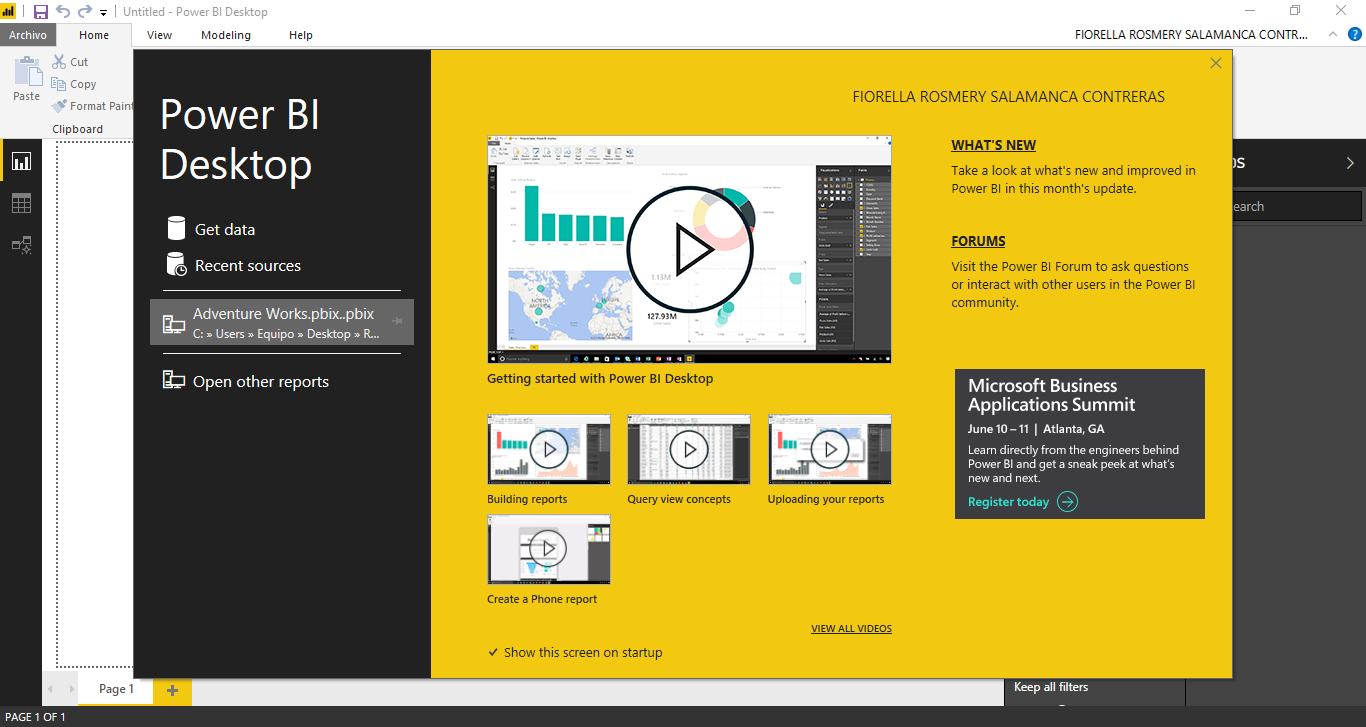
\includegraphics[width=17cm]{./Imagenes/Ejercicio1-Tarea2/1}
	\end{center}	

	\begin{center}
	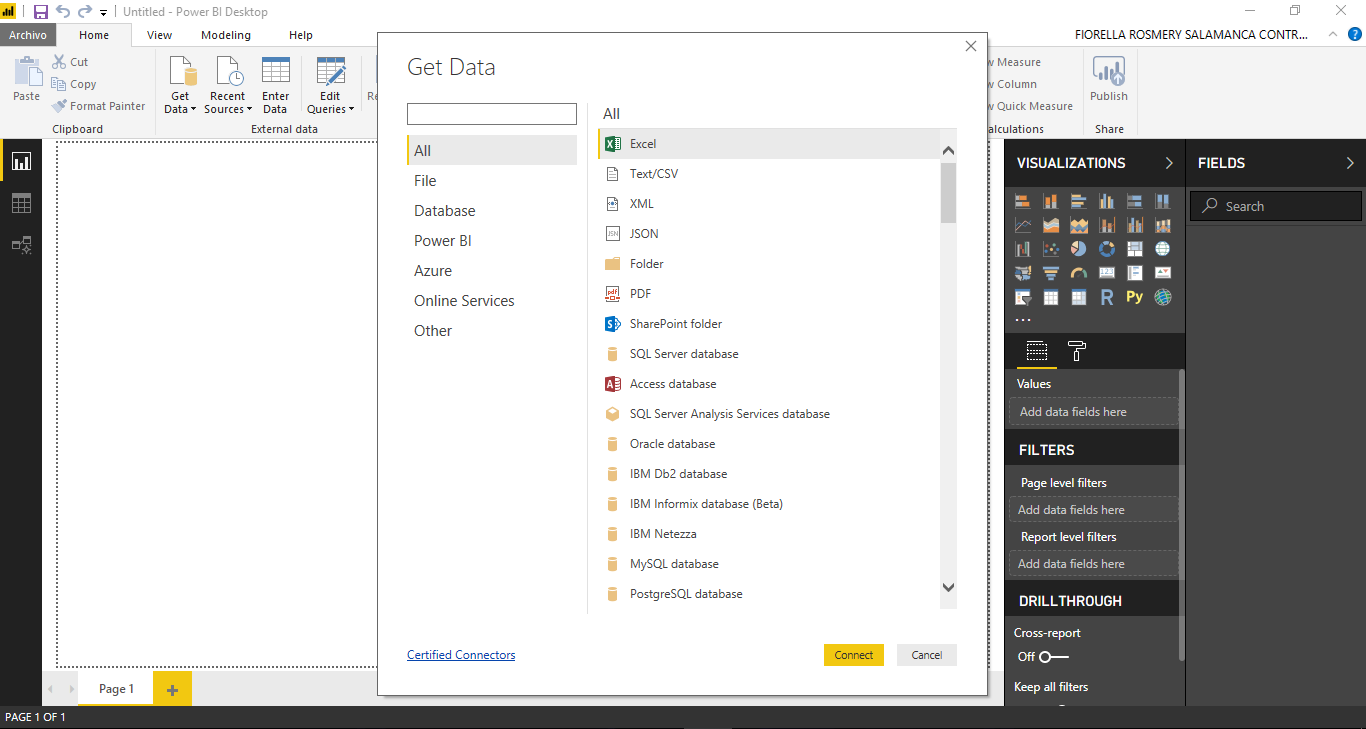
\includegraphics[width=17cm]{./Imagenes/Ejercicio1-Tarea2/2}
	\end{center}	

    \item Abrir el archivo Adventure Works Product Categories.xlsx.

	\begin{center}
	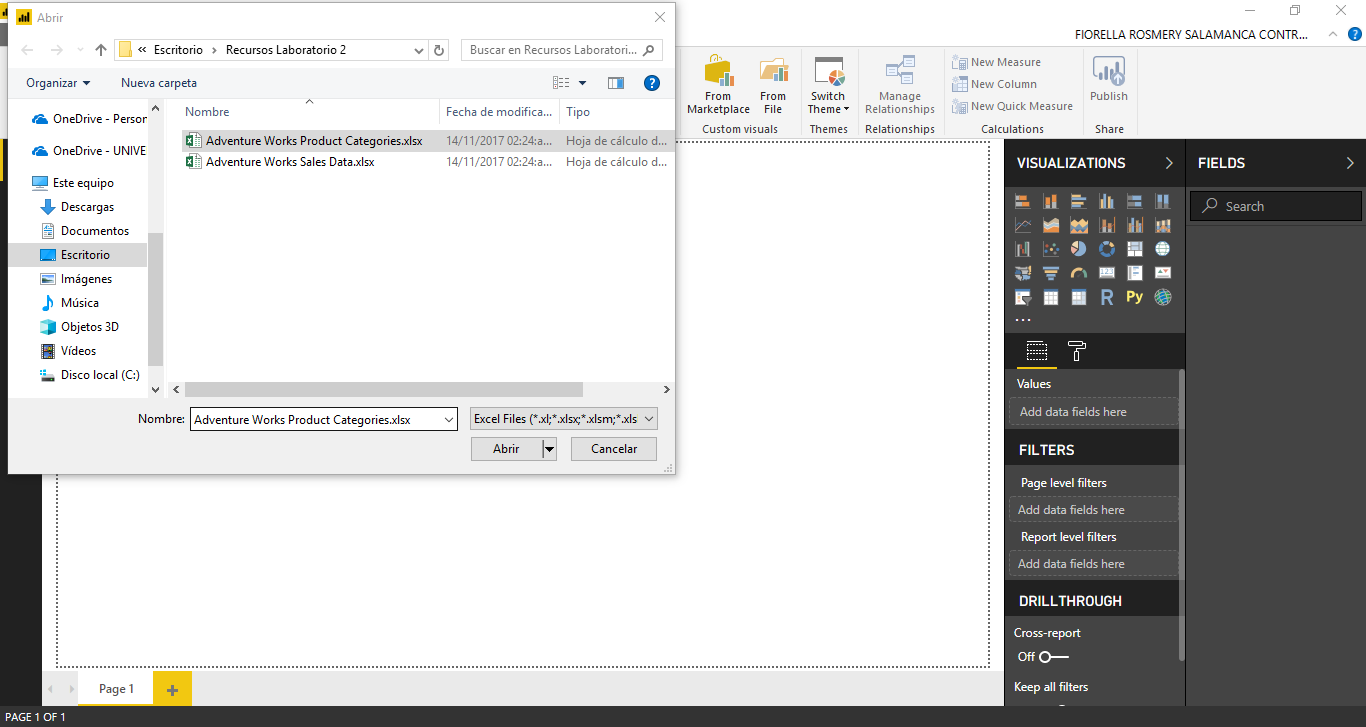
\includegraphics[width=17cm]{./Imagenes/Ejercicio1-Tarea2/3}
	\end{center}	

    \item En el cuadro de dialogo Explorador (Navigator), seleccionar las hojas DimProductCategory, and DimProductSubcategory, y luego hacer click en Cargar (Load).

	\begin{center}
	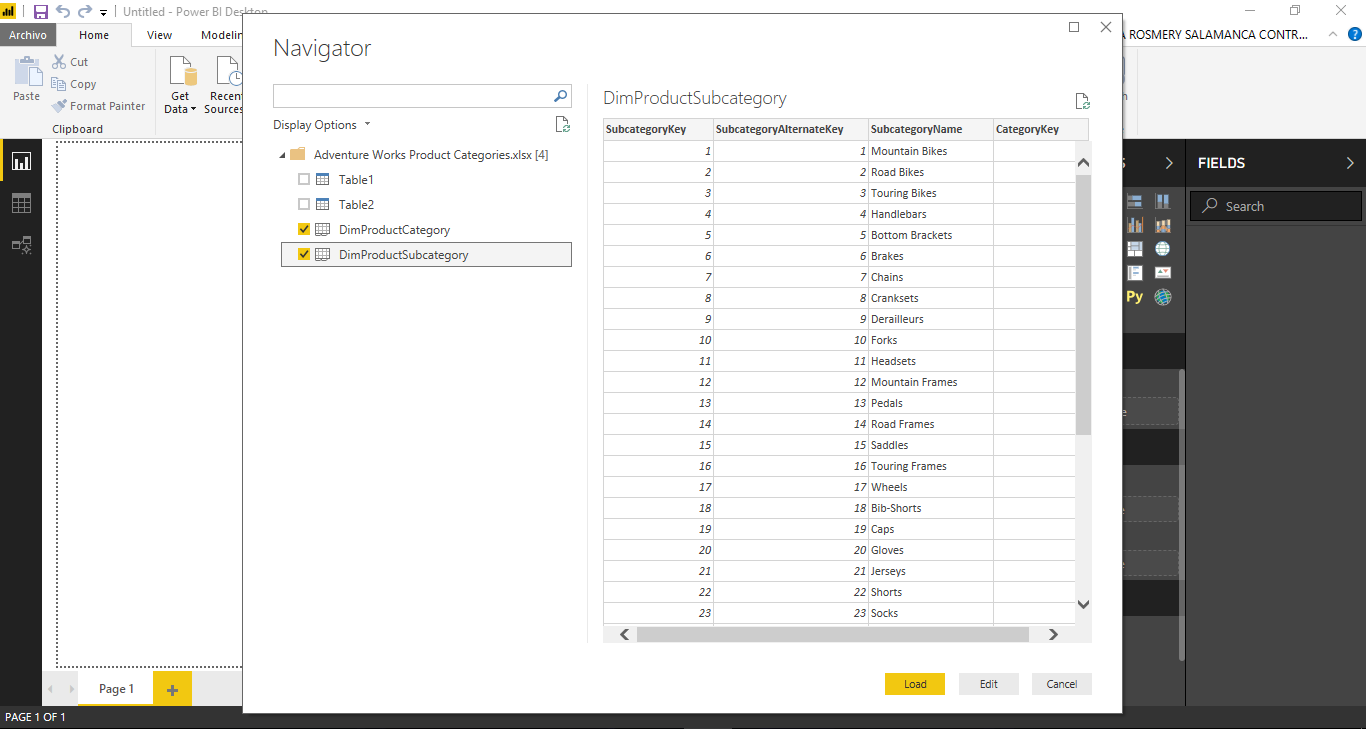
\includegraphics[width=17cm]{./Imagenes/Ejercicio1-Tarea2/4}
	\end{center}	

    \item  En el panel de Relaciones, revisar la relación que Power BI ha creado entre las dos tablas.

	\begin{center}
	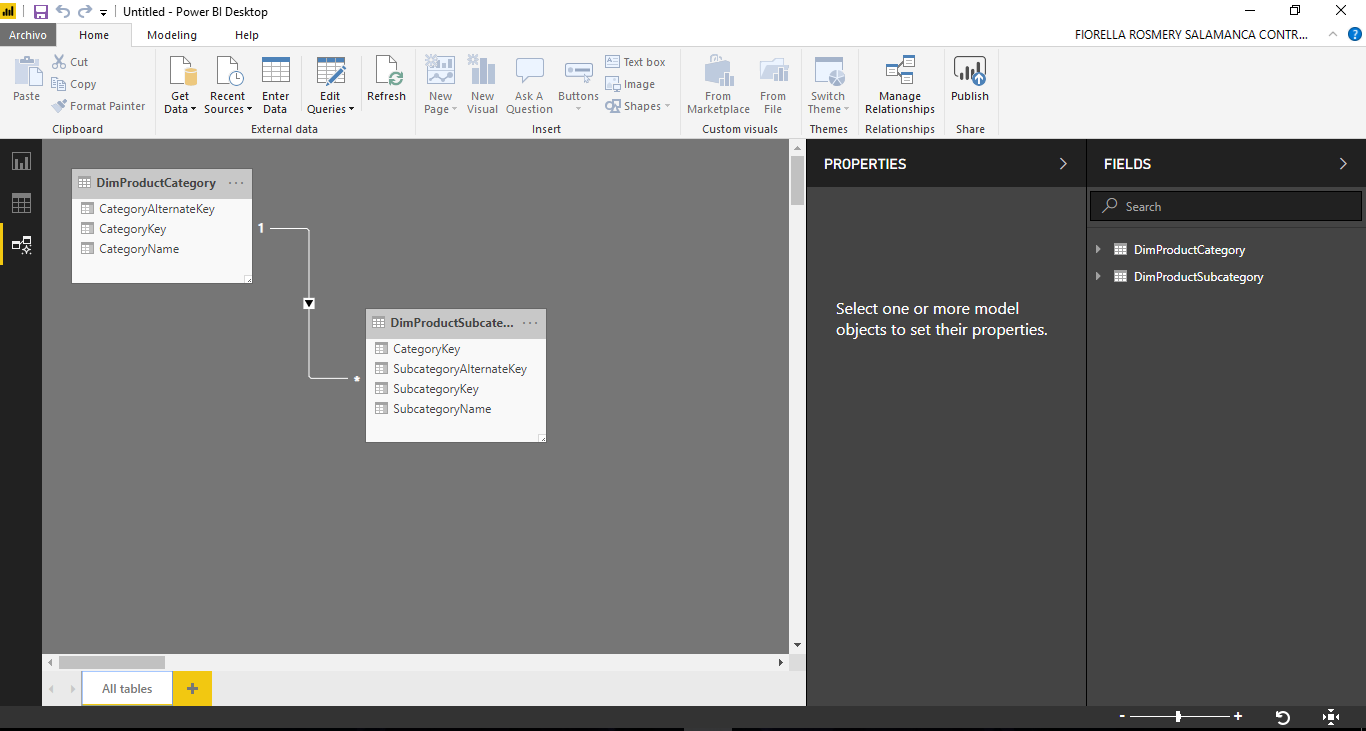
\includegraphics[width=17cm]{./Imagenes/Ejercicio1-Tarea2/5}
	\end{center}	

    \item Hacer click en la línea de la relación entre DimProductCategory, y DimProductSubcategory, y seleccionar Eliminar (Delete).
    \item En el cuadro de dialogo Eliminar relación (Delete Relationship), hacer click en Borrar (Delete).

	\begin{center}
	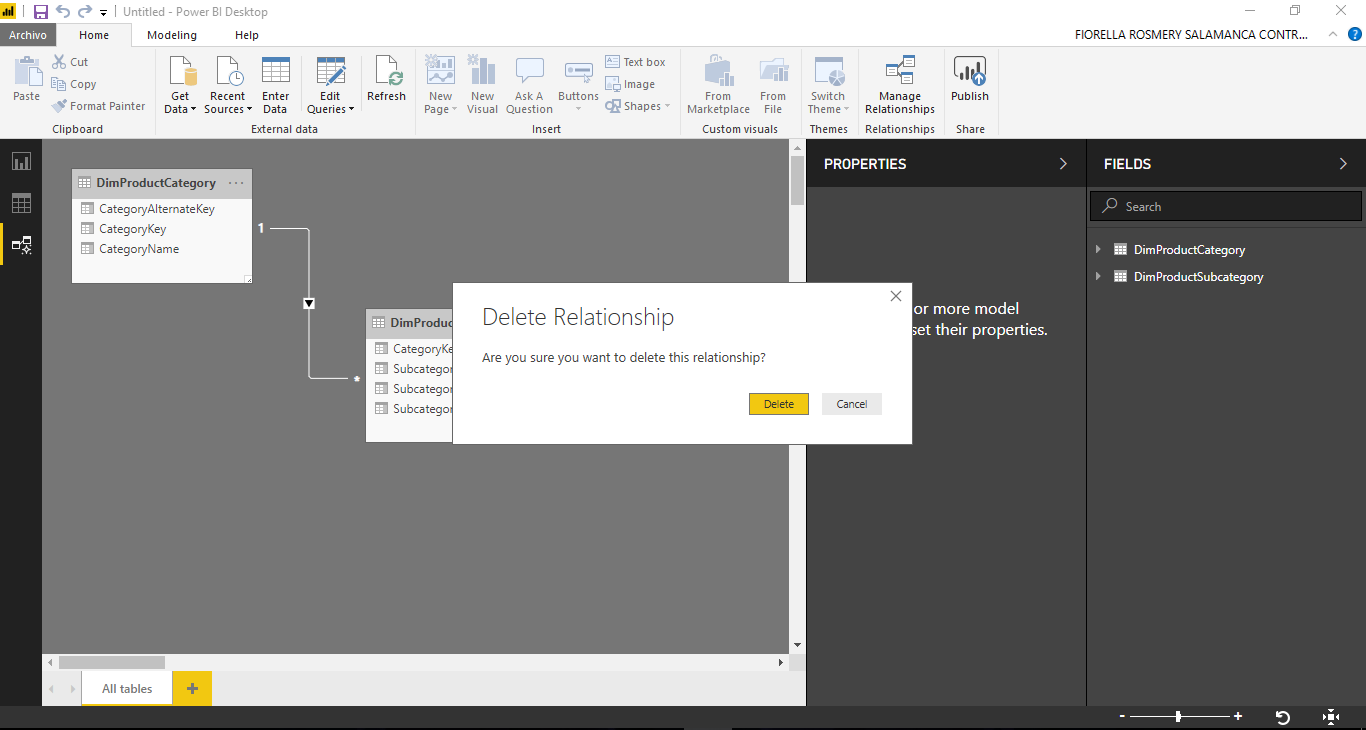
\includegraphics[width=17cm]{./Imagenes/Ejercicio1-Tarea2/6}
	\end{center}	

    \item Arrastrar la columna CategoryKey en la tabla DimProductSubcategory a la columna Category en la tabla DimProductCategory, para crear una relación Muchos a uno (Many to One (*:1)), y una dirección de filtro cruzado (Cross filter direction) en ambos.

	\begin{center}
	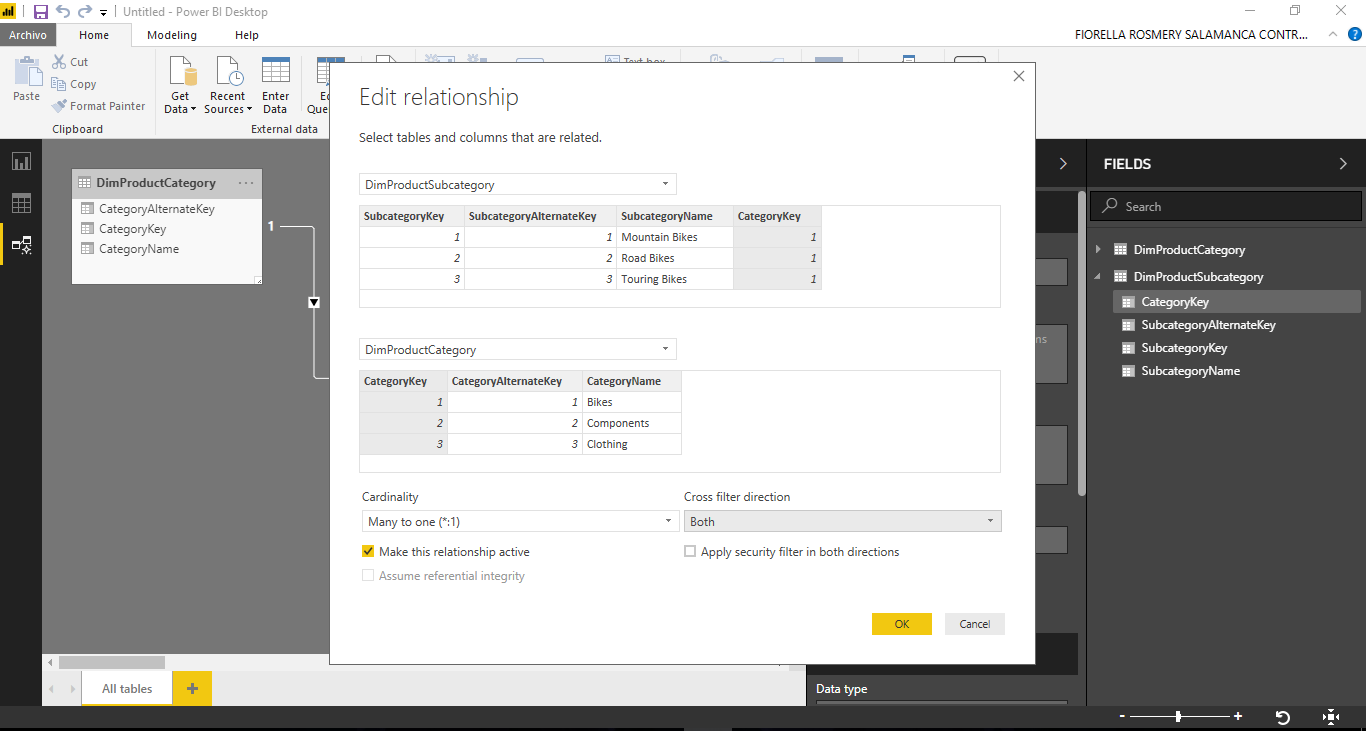
\includegraphics[width=17cm]{./Imagenes/Ejercicio1-Tarea2/7}
	\end{center}	

    \item En la tabla DimProduct, arrastrar la columna ProductSubcategoryKey a la columna SubcategoryKey en la tabla DimProductSubcategory, para crear una relación de Muchos a Uno (Many to One (*:1)), y una dirección de filtro cruzado (Cross filter direction) en ambos.

	\begin{center}
	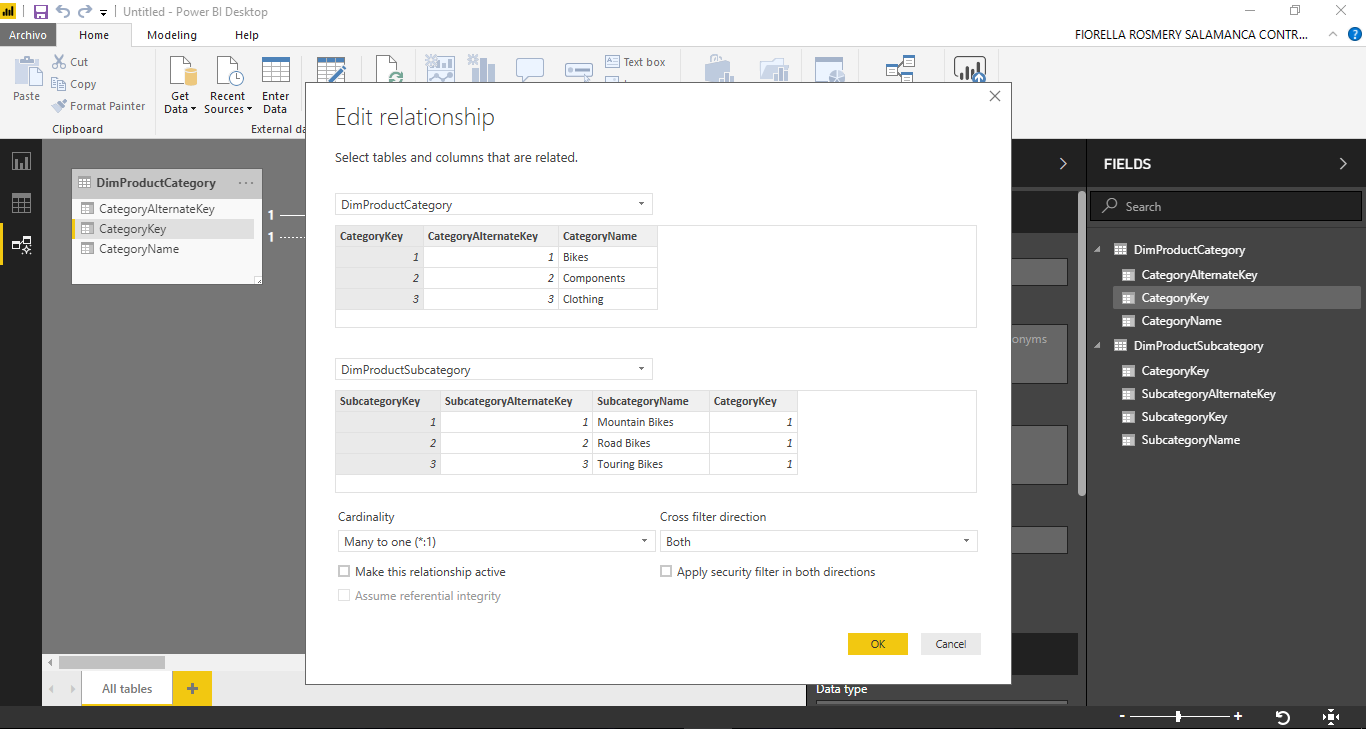
\includegraphics[width=17cm]{./Imagenes/Ejercicio1-Tarea2/8}
	\end{center}	

	\begin{center}
	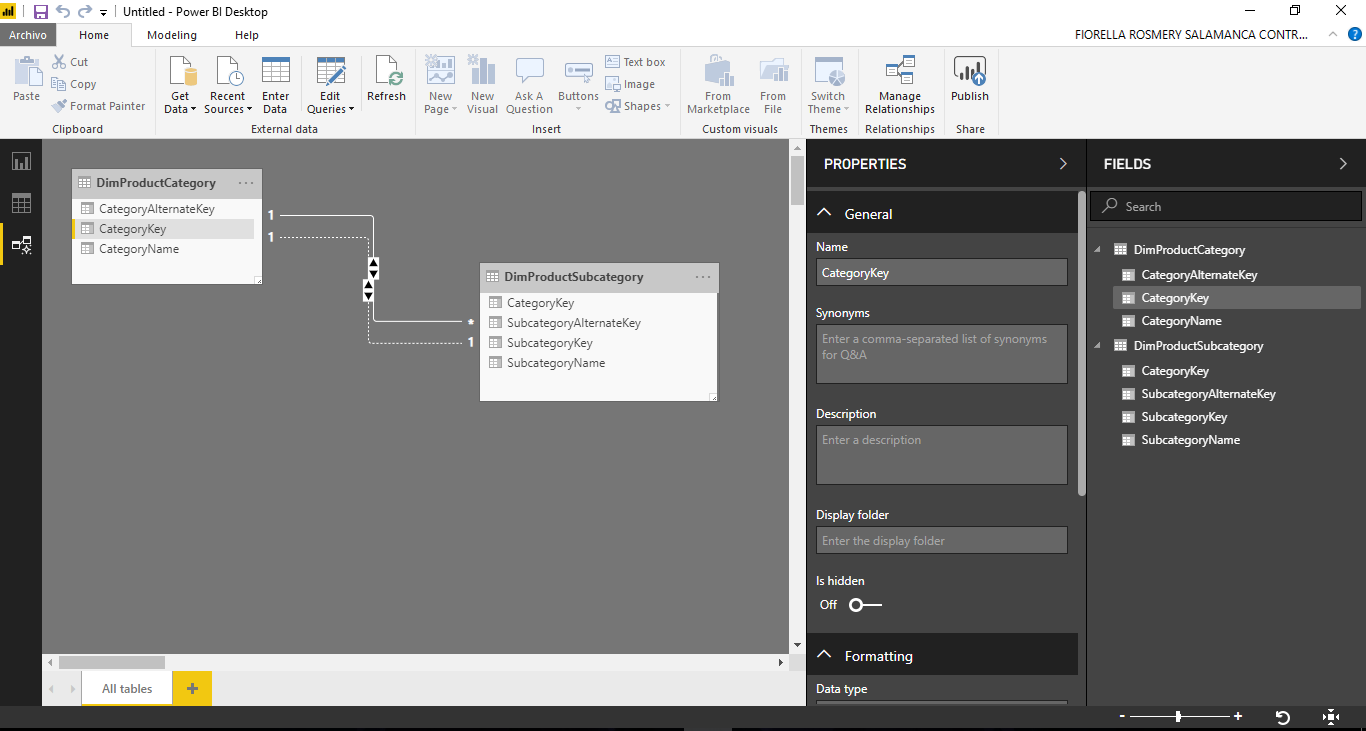
\includegraphics[width=17cm]{./Imagenes/Ejercicio1-Tarea2/9}
	\end{center}	

    \item Hacer click en Guardar.

\end{enumerate}



\section{Ejercicio 2: Calculations - Tarea 1: Añadir una Columna Calculada} 


\begin{enumerate}[1.]
    \item En Power BI Desktop, haga clic en Data en el panel de vistas en el lado izquierdo.
    \item En el panel Fields, haga clic en DimCustomer.

	\begin{center}
	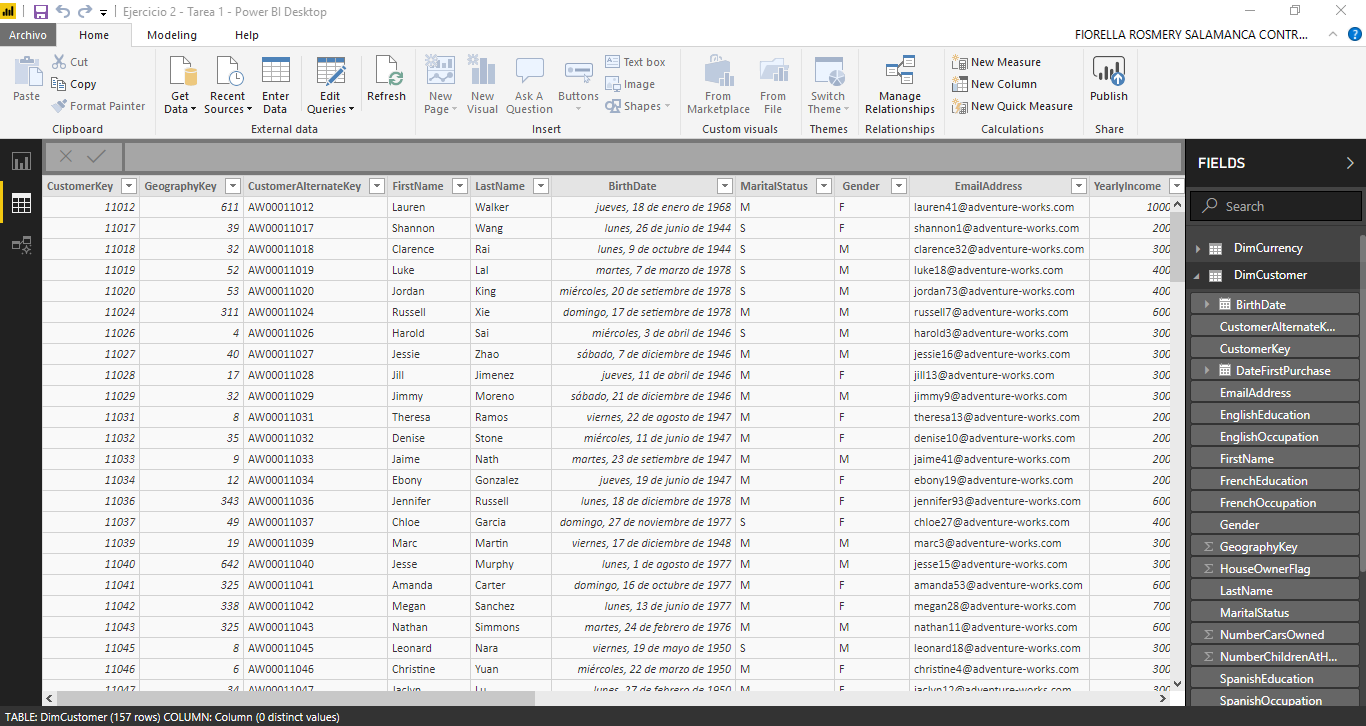
\includegraphics[width=17cm]{./Imagenes/Ejercicio2-Tarea1/1}
	\end{center}	

    \item En la cinta Modeling, en el grupo Calculations, haga clic en New Column.
    \item En la barra de fórmulas, resalte Column = y escriba:\\

\textbf {IncomeStatus = IF (DimCustomer[YearlyIncome] < 25000, "Lower Income", IF \\
(AND(DimCustomer[YearlyIncome] >= 25000, DimCustomer[YearlyIncome] < 60000), "Middle Income", IF\\ (AND(DimCustomer[YearlyIncome] >= 60000, DimCustomer[YearlyIncome] < 100000), "Higher Income", IF\\ (DimCustomer[YearlyIncome] >= 100000, "Very High Income", " Other"))))}\\

	\begin{center}
	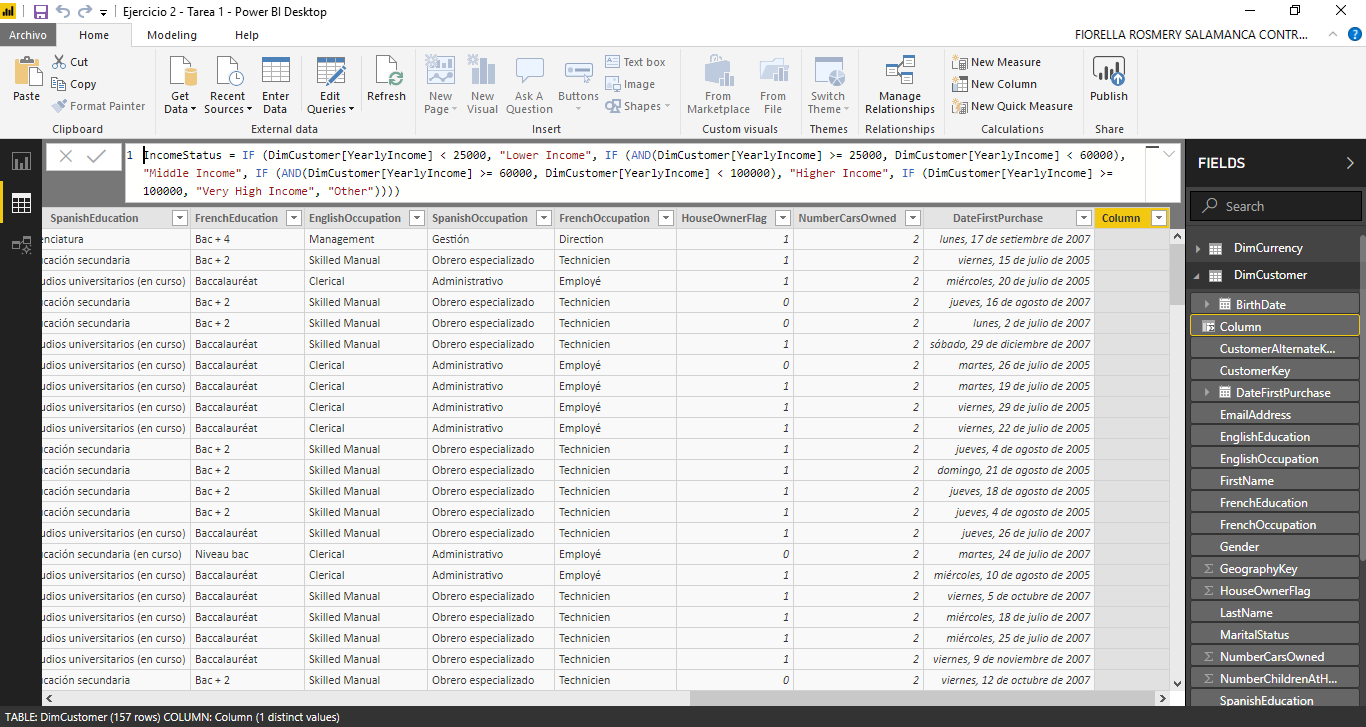
\includegraphics[width=17cm]{./Imagenes/Ejercicio2-Tarea1/2}
	\end{center}	

    \item Presione Enter.
    \item En la cinta Modeling, en el grupo Calculations, haga clic en New Column.
    \item En la barra de fórmulas, resalte Column = y escriba: \\

\textbf{DaysSinceFirstPurchase = DATEDIFF(DimCustomer[DateFirstPurchase], TODAY(), DAY)}\\

	\begin{center}
	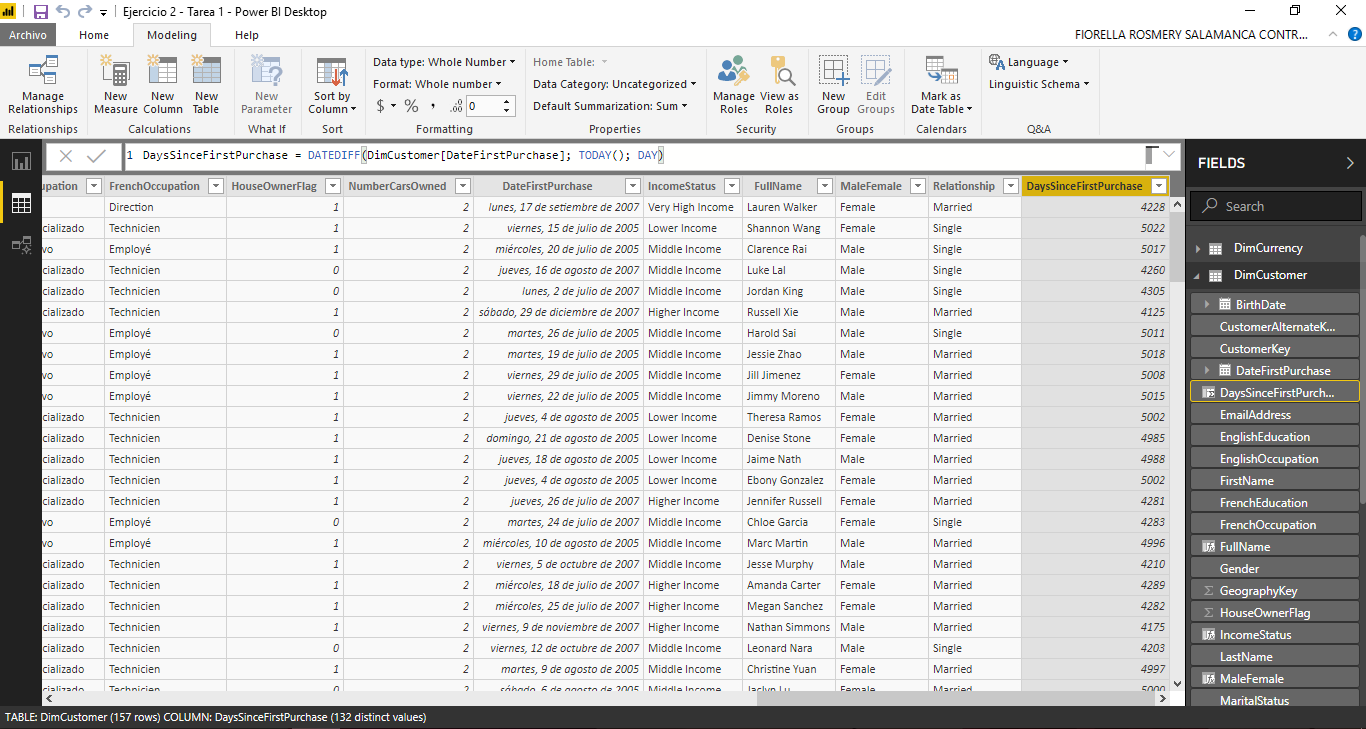
\includegraphics[width=17cm]{./Imagenes/Ejercicio2-Tarea1/22}
	\end{center}	

    \item Presione Enter.
    \item En la cinta Modeling, en el grupo Calculations, haga clic en New Column.
    \item En la barra de fórmulas, resalte Column = y escriba: \\

\textbf{FullName = [FirstName] \& " " \& [LastName]}\\

	\begin{center}
	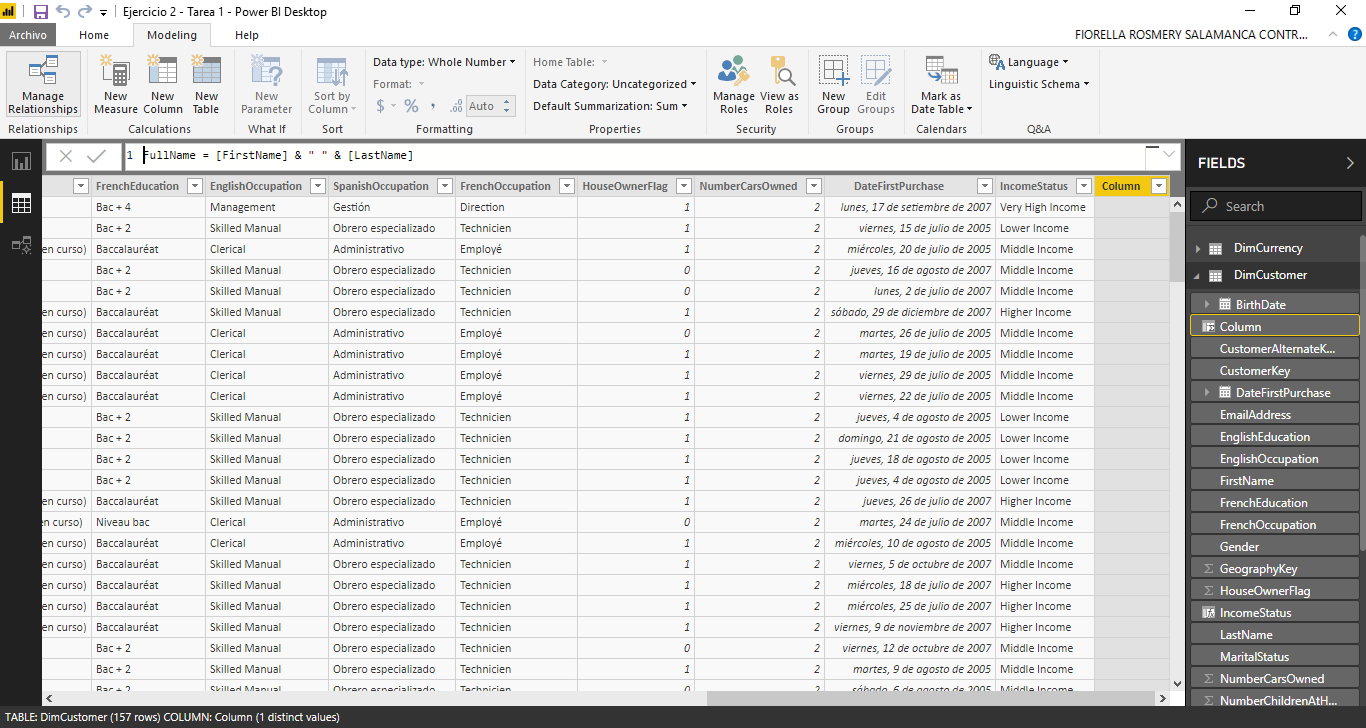
\includegraphics[width=17cm]{./Imagenes/Ejercicio2-Tarea1/3}
	\end{center}	

    \item Presione Enter.
    \item En la cinta Modeling, en el grupo Calculations, haga clic en New Column.
    \item En la barra de fórmulas, resalte Column = y escriba: \\

\textbf{MaleFemale = IF([Gender] = "M", "Male", "Female")}\\

	\begin{center}
	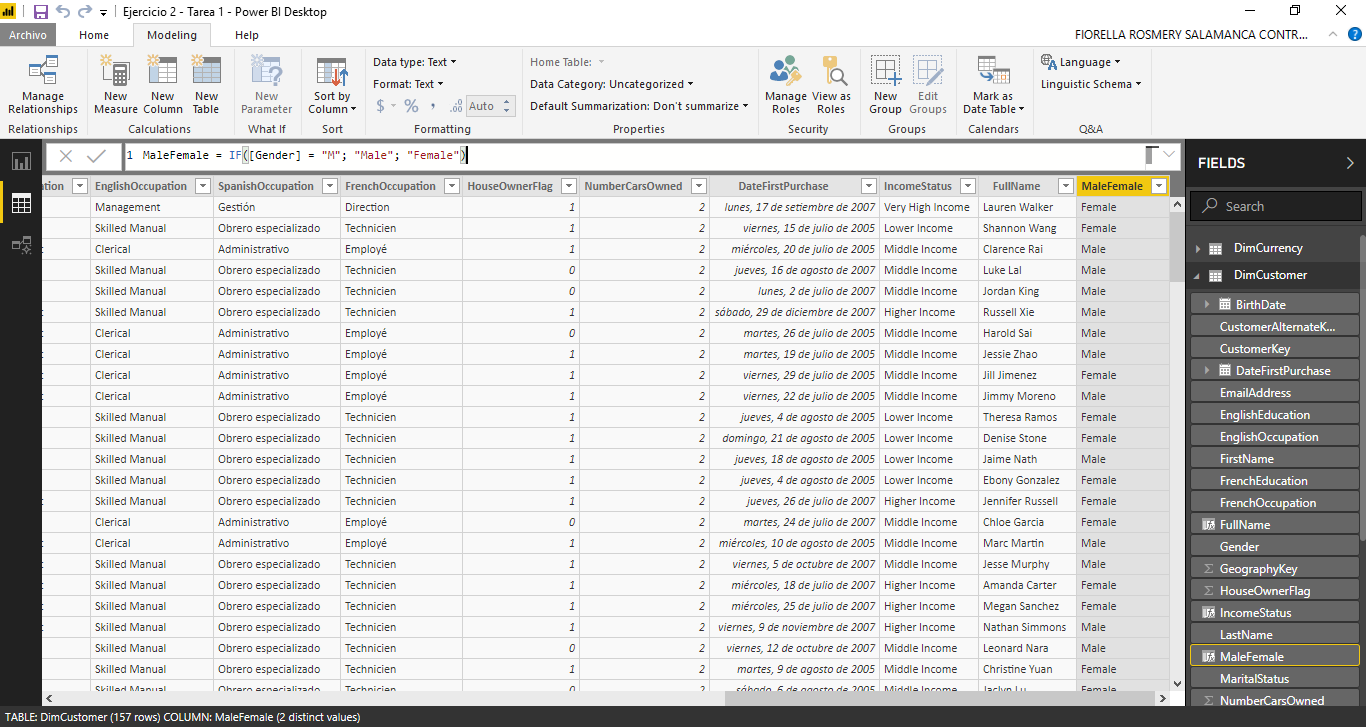
\includegraphics[width=17cm]{./Imagenes/Ejercicio2-Tarea1/4}
	\end{center}	

    \item Presione Enter.
    \item En la cinta Modeling, en el grupo Calculations, haga clic en New Column.
    \item En la barra de fórmulas, resalte Column = y escriba:\\

\textbf{Relationship = IF([MaritalStatus] = "M", "Married", "Single")}\\

	\begin{center}
	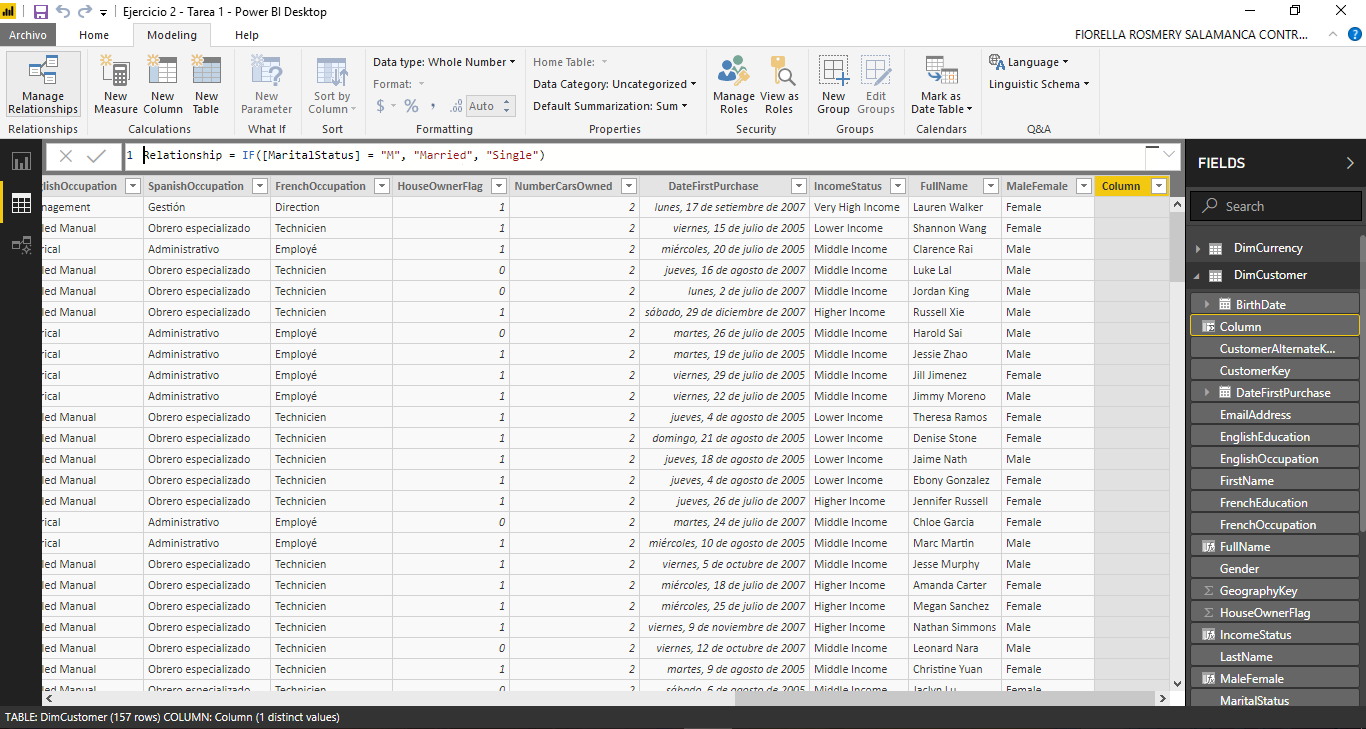
\includegraphics[width=17cm]{./Imagenes/Ejercicio2-Tarea1/5}
	\end{center}	

    \item Presione Enter.
    \item En el panel Fields, haga clic en DimProductSubcategory.
    \item En la cinta de Modeling, en el grupo Calculations, haga clic en New Column.
    \item En la barra de fórmulas, resalte Column = y escriba: \\

\textbf{MainCategory = RELATED(DimProductCategory[CategoryName])}\\

	\begin{center}
	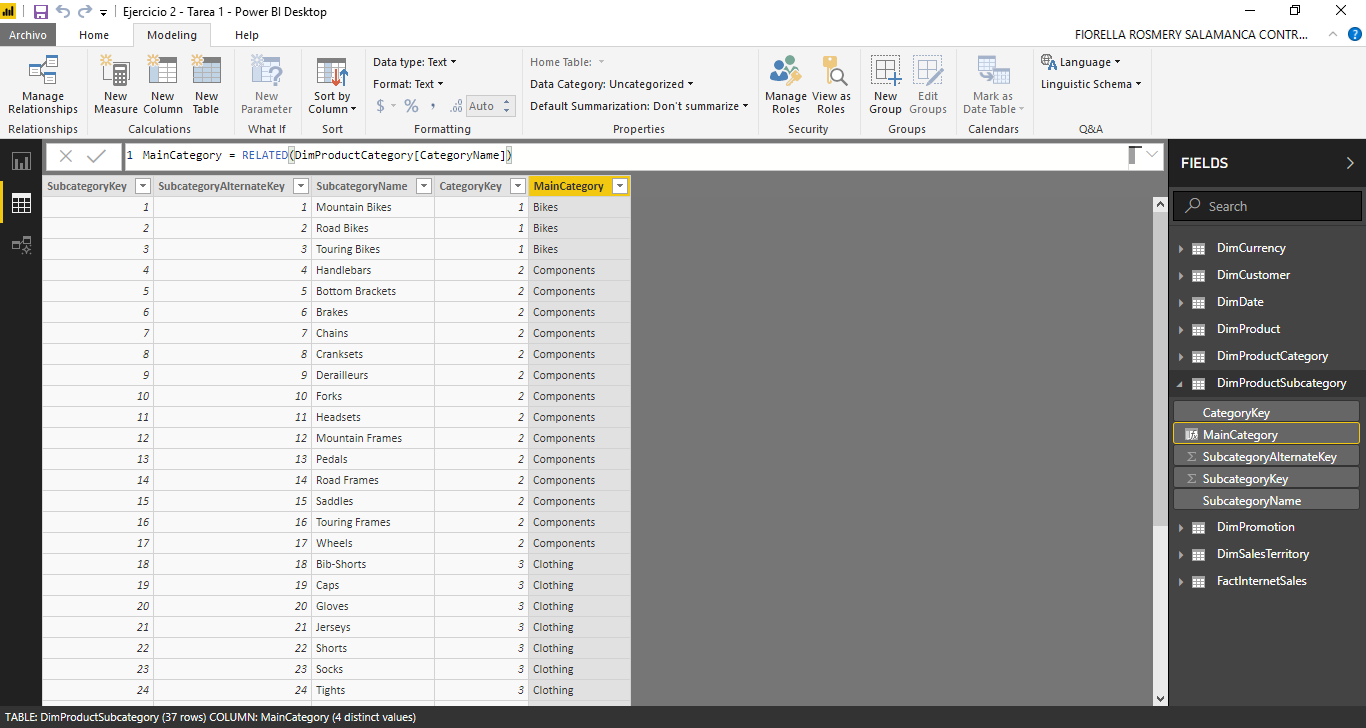
\includegraphics[width=17cm]{./Imagenes/Ejercicio2-Tarea1/6}
	\end{center}	

    \item Presione Enter.
    \item En el panel Fields, haga clic en DimPromotion.
    \item En la cinta Modeling, en el grupo Calculations, haga clic en New Column.
    \item En la barra de fórmulas, resalte Column = y escriba: \\

\textbf{PromotionLengthDays = DATEDIFF(DimPromotion[StartDate],\\
DimPromotion[EndDate], DAY)}\\

	\begin{center}
	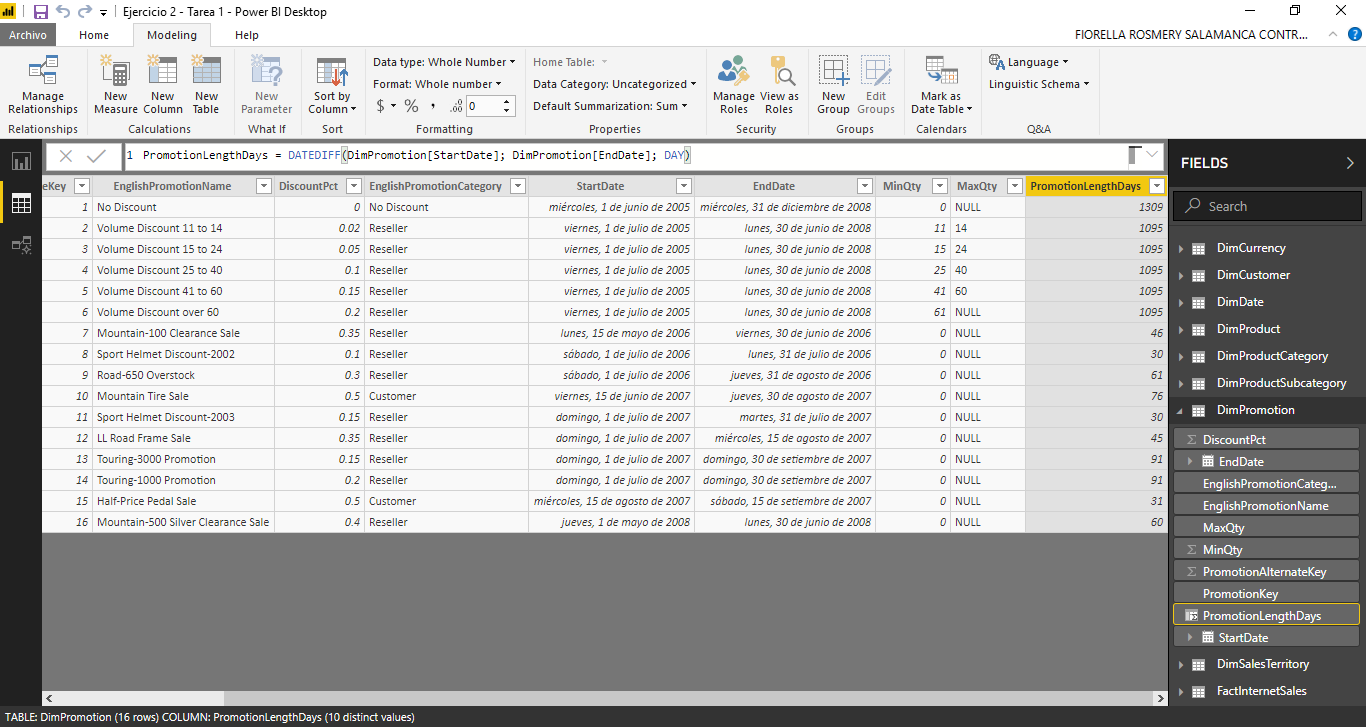
\includegraphics[width=15cm]{./Imagenes/Ejercicio2-Tarea1/7}
	\end{center}	

    \item Presione Enter.
    \item En el panel Fields, haga clic en FactInternetSales.
    \item En la cinta Modeling, en el grupo Calculations, haga clic en New Column.
    \item En la barra de fórmulas, resalte Column = y escriba: \\

\textbf{Profit = CURRENCY(FactInternetSales[UnitPrice] - \\
FactInternetSales [ProductStandardCost])}\\

	\begin{center}
	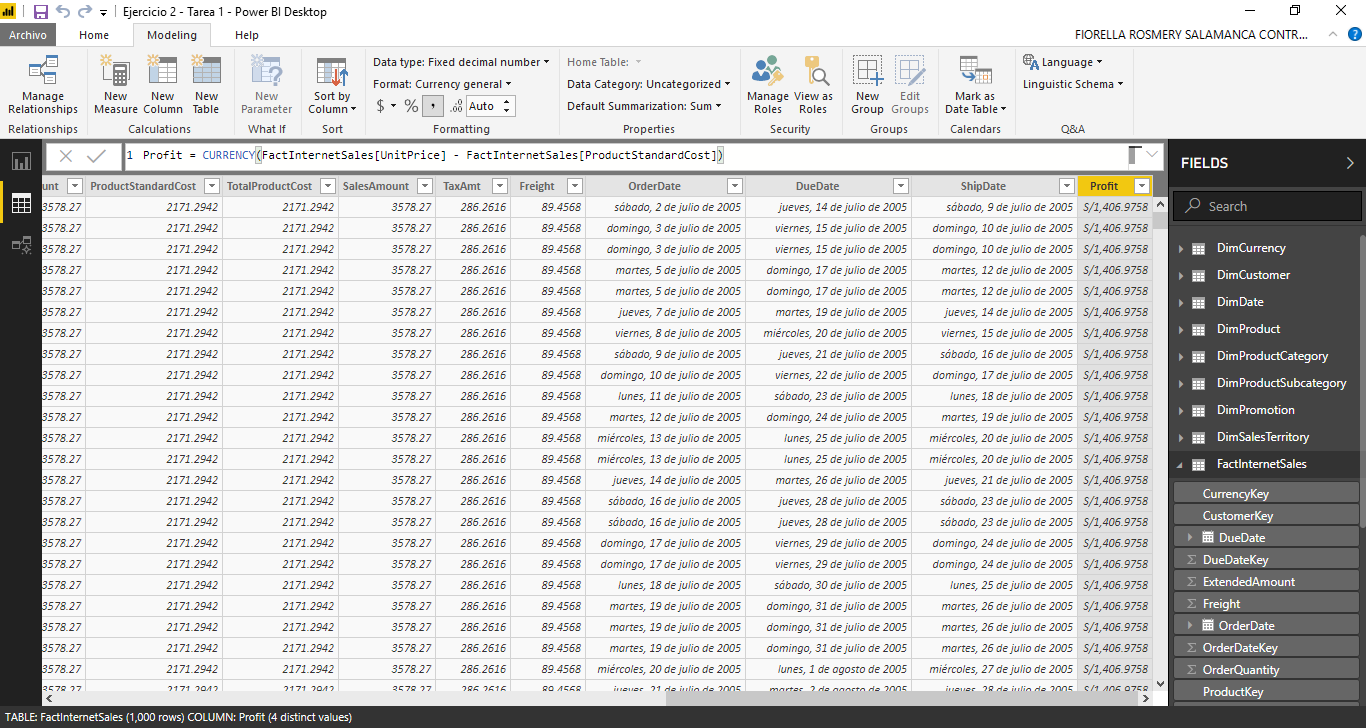
\includegraphics[width=15cm]{./Imagenes/Ejercicio2-Tarea1/8}
	\end{center}	

    \item Presionar Enter.
    \item Cerrar Power BI Desktop, salvando cualquier cambio

\end{enumerate}


\end{document}
